%%%%%%%%%%%%%%%%%%%%%%%%%%%%%%%%%%%%%%%%%
% University Assignment Title Page 
% LaTeX Template
% Version 1.0 (27/12/12)
%
% This template has been downloaded from:
% http:\\www.LaTeXTemplates.com
%
% Original author:
% WikiBooks (http:\\en.wikibooks.org/wiki/LaTeX/Title_Creation)
%
% License:
% CC BY-NC-SA 3.0 (http:\\creativecommons.org/licenses/by-nc-sa/3.0/)
% %%%%%%%%%%%%%%%%%%%%%%%%%%%%%%%%%%%%%%%%
\documentclass[12pt]{article}
\usepackage{tabularx}
\usepackage[hidelinks]{hyperref}
\hypersetup{linktoc=all}
\usepackage{graphicx}

\usepackage{pdfpages}

\begin{document}
\sloppy

\begin{titlepage}

\newcommand{\HRule}{\rule{\linewidth}{0.5mm}} % Defines a new command for the 
%horizontal lines, change thickness heReve

\center % Center everything on the page
 
%----------------------------------------------------------------------------------------
%	HEADING SECTIONS
%----------------------------------------------------------------------------------------

\textsc{\LARGE McMaster University}\\[1.5cm] % Name of your university/college
\textsc{\Large Software Project Management}\\[0.5cm] % Major heading such as course name
\textsc{\large SFWR ENG 3XA3}\\[0.5cm] % Minor heading such as course title

%----------------------------------------------------------------------------------------
%	TITLE SECTION
%----------------------------------------------------------------------------------------

\HRule \\[0.4cm]
{ \huge \bfseries Design Document}\\[0.4cm] % Title of your document
\HRule \\[1.5cm]
 
%----------------------------------------------------------------------------------------
%	AUTHOR SECTION
%----------------------------------------------------------------------------------------



% If you don't want a supervisor, uncomment the two lines below and remove the section above
\Large \emph{Authors:}\\
Mohammad \textsc{Naveed} \textbf{1332196} \\ % Your name
Josh \textsc{Voskamp} \textbf{1319352} \\
Stephan \textsc{Arulthasan} \textbf{1308004} \\[3cm]
%----------------------------------------------------------------------------------------
%	DATE SECTION
%----------------------------------------------------------------------------------------

{\large \today}\\[3cm] % Date, change the \today to a set date if you want to be precise

%----------------------------------------------------------------------------------------
%	LOGO SECTION
%----------------------------------------------------------------------------------------

%\includegraphics{Logo}\\[1cm] % Include a department/university logo - this will require the graphicx package
 
%----------------------------------------------------------------------------------------

\vfill % Fill the rest of the page with whitespace

\end{titlepage}
\newpage
\tableofcontents
\newpage
\listoftables
\addcontentsline{toc}{section}{List of Tables}
\newpage
\listoffigures
\addcontentsline{toc}{section}{List of Figures}
\newpage

\section*{Revision History}
\addcontentsline{toc}{section}{Revision History}
\begin{table}[!htbp]
	\centering
	\begin{tabular}{ | p{2cm} | p{2cm}| p{6cm} | p{4cm}|}
		\hline
		Rev. No. & Rev. Date & Description & Author \\\hline
		0 & Nov 2 2015 & Created Document & Mohammad Naveed \\\hline
		0 & Nov 2 2015 & Added Module Hierarchy & Josh Voskamp \\\hline
		0 & Nov 4 2015 & Added Module Decomposition & Stephan Arulthasan\\\hline
		0 & Nov 4 2015 & Added Introduction & Mohammad Naveed \\\hline
		0 & Nov 4 2015 & Improved Module Hierarchy & Josh Voskamp \\\hline
		0 & Nov 4 2015 & Added Anticipated Changes & Mohammad Naveed \\\hline
		0 & Nov 4 2015 & Improved Module Decomposition & Stephan Arulthasan \\\hline
		0 & Nov 6 2015 & Added Uses Hierarchy Diagram & Josh Voskamp \\\hline
		0 & Nov 6 2015 & Completed Traceability Matrix & Stephan Arulthasan \\\hline
		
	\end{tabular}
	\caption{Revision History}
\end{table}
\newpage

\section{Introduction}
According to Jane McGonigal, a well known and world renowned game 
designer; we spend 3 billion hours a week playing video games. That is a lot of 
time that many people argue could be spent better, and that is what 2048 aims to 
accomplish. More and more people are playing video games everyday and 
2048 is a fun and challenging game that tests the users? mathematical as well as 
their spatial intelligence. This allows 2048 to be fun, yet still be brain 
enhancing. Since the target audience for this game is so large, we can take 
advantage of this by providing users an option to spend their gaming time in a way 
thats beneficial mentally while still being entertained. \par
The design pattern that will be used to implement 2048 is the Model View Controller (MVC) design pattern. This pattern is based on the decomposition of the software into three different modules. The decomposition is based on the concept of information hiding. The model, view and controller modules. Each module has a specific task that it needs to focus on, for example, the view module focuses on the GUI of the game whereas the model module focuses on the data structures and actual data used in the game. \par
In terms of other documentation, after completing the Software Requirements Specification (SRS), the first part of the design document is completed which is then followed by the development of the Module Interface Specification (MIS). The MIS specifies the externally observable behaviour of a module's access routines. \par
The rest of the design document is organized as follows, section 2 lists the anticipated and unlikely changes of the software requirements. Section 3 lists the module hierarchy that was constructed. Section 4 lists the connection between requirements and design. Section 5 includes two traceability matrices that check the completeness of the requirements provided in the SRS. Section 6 gives a detailed description of the modules. Section 7 describes the use relation between modules. 

\section{Anticipated and Unlikely Changes}
This section lists possible changes to the system that are put into two sections, according to their likelihood. The first subsection are the anticipated changes(section 2.1), and the second subsection are the unlikely changes(section 2.2).
\subsection{Anticipated Changes}
Anticipated changes are the source of the information that is to be hidden inside the modules.
Ideally, changing one of the anticipated changes will only require changing the one module
that hides the associated decision. The approach adapted here is called design for change.
\begin{itemize}
\item \textbf{AC1:} The hardware the game will run on
\item \textbf{AC2:} Winning tile needed to finish the game
\item \textbf{AC3:} Size of the board
\item \textbf{AC4:} Number on largest tile
\item \textbf{AC5:} High score section
\item \textbf{AC6:} The OS the software will run on
\end{itemize}

\subsection{Unlikely Changes}
It is not intended that the following changes will be made because if they were to be changed, then many parts of the design must be modified. Therefore instead of having to modify the rest of the modules and making the implementation more difficult, the changes listed below are unlikely in order to keep the design consistent and robust. 
\begin{itemize}
\item \textbf{UC1:} Input to the game
\item \textbf{UC2:} Smallest tile to start the game
\item \textbf{UC3:} Moves allowed
\item \textbf{UC4:} Output of the game
\item \textbf{UC5:} Progress through game (i.e. similar tiles are added not multiplied)
\item \textbf{UC6:} Scoring mechanism
\item \textbf{UC7:}  Losing conditions 
\end{itemize} 

\section{Module Hierarchy}
This section provides an overview of the module design. Modules are summarized 
in a hierarchy decomposed by secrets in Table 1. The modules listed below, 
which are leaves in the hierarchy tree, are the modules that will actually be 
implemented.\bigskip\\
\textbf{M1:} Hardware-Hiding Module \\
\textbf{M2:} Keyboard \\
\textbf{M3:} GameView\\
\textbf{M4:} Main\\
\textbf{M5:} Board\\
\textbf{M6:} Tile\\

\begin{table}[!htbp]
	\centering
	\begin{tabular}{p{5cm}|p{4cm}|p{4cm}}
		\textbf{Level 1} & \textbf{Level 2} & \textbf{Level 3} \\\hline
		Hardware-Hiding Module & \\\hline
		Behaviour-Hiding Module & Keyboard & \\
		& GameView & \\
		& Main & \\\hline
		Software Decision Module & Board & Tile\\\hline
		
	\end{tabular}
	\smallskip
	\caption{Module Hierarchy}
	\label{Module Hierarchy}	
\end{table}

\section{Connection Between Requirements and Design}
The design of the system is intended to satisfy the requirements developed in the SRS. In this stage, the system is decomposed into modules. The connection between requirements and modules is listed in Table 3.

\section{Module Decomposition}
Modules are decomposed according to the principle of "information hiding". Each module hides some design decision from the rest of the system. This is described in the \textit{Secrets} field. The \textit{Services} field specifies \textit{what} the module will do without documenting \textit{how} to do it. Only the leaf modules in the hierarchy have to be implemented. If a dash (\emph{--}) is shown, this means that the module is not a leaf and will not have to be implemented. Whether or not this module is implemented depends on the programming language selected.

\subsection{Hardware Hiding Modules \textbf{M1}}

\begin{description}
\item[Secrets:]The data structure and algorithm used to implement the virtual
  hardware.
\item[Services:]Serves as a virtual hardware used by the rest of the
  system. This module provides the interface between the hardware and the
  software. So, the system can use it to display outputs or to accept inputs.
\item[Implemented By:] OS
\end{description}

\subsection{Behaviour-Hiding Module}

\begin{description}
\item[Secrets:]The contents of the required behaviors.
\item[Services:]Includes programs that provide externally visible behavior of
  the system as specified in the software requirements specification (SRS)
  documents. This module serves as a communication layer between the
  hardware-hiding module and the software decision module. The programs in this
  module will need to change if there are changes in the SRS.
\item[Implemented By:] --
\end{description}

\subsubsection{Keyboard \textbf{M2}}

\begin{description}
\item[Secrets:]The format and structure of the input data
\item[Services:]Converts the input data into the data structure used by the
  input parameters module.
\item[Implemented By:] 2048
\end{description}

\subsubsection{GameView \textbf{M3}}

\begin{description}
\item[Secrets:]The format and structure of the output data.
\item[Services:]Outputs the results of the moves, including the score, winning game, losing game, current state of the board, and notifies you about the option to restart the game when you lose. 
\item[Implemented By:] 2048
\end{description}

\subsubsection{Main \textbf{M4}}

\begin{description}
\item[Secrets:] The algorithm for coordinating the running of the program.
\item[Services:] Provides the main program.
\item[Implemented By:] 2048
\end{description}

\subsection{Software Decision Module}

\begin{description}
\item[Secrets:] The design decision based on game logic, physical
  facts, or programming considerations. The secrets of this module are
  \emph{not} described in the SRS.
\item[Services:] Includes data structure and algorithms used in the system that
  do not provide direct interaction with the user. 
\item[Implemented By:] --
\end{description}

\subsubsection{Board \textbf{M5}}

\begin{description}
\item[Secrets:] The algorithm used to run the game and create moves- also includes algorithm to win and lose the game.
\item[Services:] Provides the ability to play the game and set parameters to win and lose the game. 
\item[Implemented By:] 2048
\end{description}

\subsubsection{Tile \textbf{M6}}

\begin{description}
\item[Secrets:] The algorithm that sets the value and colour of game pieces.
\item[Services:] Provides the ability to create moves in the game and visually recognize different game pieces.
\item[Implemented By:] 2048
\end{description}


\section{Traceability Matrix}
This section shows two traceability matrices: between the modules and 
the 
requirements and between the modules and the anticipated changes. 
\smallskip
\begin{table}[!htbp]
	\centering
	\begin{tabular}{p{3cm}|p{9cm}}
		\textbf{Req.} & \textbf{Modules} \\\hline
		R1 & M1, M3, M4\\
		R2 & M1, M3, M4 \\
		R3 & M1, M3, M4 \\
		R4 & M1, M2, M3, M4, M5, M6 \\
		R5 & M1, M2, M3, M4, M5, M6\\
		R6 & M1, M2, M3, M4, M5, M6\\
		R7 & M1, M2, M3, M4, M5, M6\\
		R8 & M1, M2, M3, M4, M5, M6\\\hline
	\end{tabular}
	\caption{Trace Between Requirements and Modules}
	\label{Trace Between Requirements and Modules}
\end{table}
\begin{table}[!htbp]
	\centering
	\begin{tabular}{p{3cm}|p{9cm}}
		\textbf{AC} & \textbf{Modules} \\\hline
		AC1 & M1 \\ 
		AC2 &  M6\\  
		AC3 &  M5\\  
		AC4 &  M6\\ 
		AC5 & M3\\ 
		AC6 & M1\\ \hline
	\end{tabular}
	\caption{Trace Between Anticipated Changes and Modules}
	\label{Trace Between Anticipated Changes and Modules}
\end{table}
\newpage

\section{Use Hierarchy Between Modules}
\begin{figure}[!htbp]
	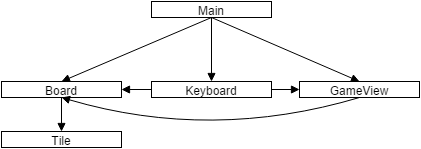
\includegraphics{uses}
	\centering
	\caption{Uses Hierarchy Diagram}
	\label{Uses Hierarchy Diagram}
\end{figure}

\section {Project Plan}
\href{run:Gantt_Chart.pdf}{Refer to Gantt Chart.pdf}\\
\href{run:Pert_Chart.pdf}{Refer to Pert Chart.pdf}\\
\href{run:Timeline.pdf}{Refer to Timeline.pdf}\\

\end{document}

